% !Mode:: "TeX:UTF-8"
% !TEX program  = xelatex
% !BIB program  = biber
\documentclass[AutoFakeBold,AutoFakeSlant,language=english,degree=bachelor,zihao=-4]{sustechthesis}
% 1. AutoFakeBold 与 AutoFakeSlant 为伪粗与伪斜,如果本机上有相应粗体与斜体字体,请使用 xeCJK 宏包进行设置,例如:
%   \setCJKmainfont[
%     UprightFont = * Light,
%     BoldFont = * Bold,
%     ItalicFont = Kaiti SC,
%     BoldItalicFont = Kaiti SC Bold,
%   ]{Songti SC}
%
% 2. language=chinese 基于为 ctexart 文类提供的中文排版方案修改,如果使用英文进行论文创作,请使用 language=english 选项。
%
% 3. degree=bachelor 为 sustechthesis 文类提供的本科生毕业论文模板,其他可选项为 master 与 doctor,但是均未实现,如果您对此有兴趣,欢迎 PR。
%
% 4. sustechthesis.cls 文类主要参考自去年完成使命的 sustechthesis.tex,在这一年的时间,作者的 TeX 风格与常用宏包发生许多变化,因为之前的思想为仅提供必要的格式修改相关代码,所以转换为文类形式所进行的修改较少,而近期的风格与常用宏包均体现在以下的例子文件中。
%
% 5. 示例文件均放置于相应目录的 examples 文件夹下,构建自己论文时可暂时保留,用以检索接口与使用方法。
%
% 6. 英文目录需要居中可以使用:\renewcommand{\contentsname}{\centerline{Content}}
%
% 7. LaTeX 中公式编号括号样式及章节关联的方法:https://liam.page/2013/08/23/LaTeX-Formula-Number/

% !Mode:: "TeX:UTF-8"
% !TEX program  = xelatex

% 数学符号与环境
\usepackage{amsmath,amssymb}
  \newcommand{\dd}{\mathrm{d}}
  \newcommand{\RR}{\mathbb{R}}
  \newtheorem{definition}{Definition}
  \newtheorem{problem}{Problem}
% 参考文献
\usepackage[sorting=none, style=gb7714-2015, backend=bibtex]{biblatex}
  \addbibresource{ref.bib}
% 无意义文本
\usepackage{zhlipsum,lipsum}
% 列表环境设置
\usepackage{enumitem}
% 浮动题不越过 \section
\usepackage[section]{placeins}
% 超链接
\usepackage{hyperref}
% 图片,子图,浮动题设置
\usepackage{graphicx,subcaption,float}
% 抄录环境设置,更多有趣例子请命令行输入 `texdoc tcolorbox`
\usepackage{tcolorbox}
  \tcbuselibrary{xparse}
  \DeclareTotalTCBox{\verbbox}{ O{green} v !O{} }%
    {fontupper=\ttfamily,nobeforeafter,tcbox raise base,%
    arc=0pt,outer arc=0pt,top=0pt,bottom=0pt,left=0mm,%
    right=0mm,leftrule=0pt,rightrule=0pt,toprule=0.3mm,%
    bottomrule=0.3mm,boxsep=0.5mm,bottomrule=0.3mm,boxsep=0.5mm,%
    colback=#1!10!white,colframe=#1!50!black,#3}{#2}%
\tcbuselibrary{listings,breakable}
  \newtcbinputlisting{\Python}[2]{
    listing options={language=Python,numbers=left,numberstyle=\tiny,
      breaklines,commentstyle=\color{white!50!black}\textit},
    title=\texttt{#1},listing only,breakable,
    left=6mm,right=6mm,top=2mm,bottom=2mm,listing file={#2}}
% 三线表支持
\usepackage{booktabs}

% LaTeX logo
\usepackage{hologo}
 % 导言区
% !Mode:: "TeX:UTF-8"
% !TEX program  = xelatex
\设置信息{
%   键 = {{中文值}, {英文值}},
    分类号 = {{}, {}},
    编号 = {{}, {}},
    UDC = {{}, {}},
    密级 = {{}, {}},
    题目 = {{Traffic State Prediction}, {Traffic State Prediction}},
    副标题 = {{崔氏集团实验室}, {CUI Inc. Lab}},
    姓名 = {{董正}, {Zheng Dong}},
    学号 = {{11812804}, {11812804}},
    系别 = {{计算机科学与工程系}, {Computer Science and Engineering}},
    专业 = {{计算机科学与技术}, {Computer Science and Technology}},
    指导老师 = {{宋轩}, {Xuan Song}},
    时间 = {{2022年3月16日}, {March 16, 2022}},
    职称 = {{研究员}, {yan jiu yuan}},
}
 % 论文信息
\begin{document}

% \中文标题页\英文标题页

% \中文诚信承诺书
% \英文诚信承诺书

% \前序格式化
% \摘要标题
% % !Mode:: "TeX:UTF-8"
% !TEX program  = xelatex
\begin{中文摘要}{关键词;关键词}
  啊啊啊啊啊啊啊啊\footnote{???}
\end{中文摘要}

\begin{英文摘要}{kw, kw}
  aaaaaaaaaaaaaaaaaaaaaaaa
\end{英文摘要} % 论文摘要

\目录\clearpage % 目录及换页

\正文格式化

\section{Introduction}
With the great development of modern cities, the rapid growth of population and the acceleration of urbanization has made transportation systems to an essential infrastructure. In the meantime, transportation systems are becoming more and more complex, which causes great pressure on urban traffic management. As a result, it is important to develop the Intelligent Transportation System (ITS)\cite{ITS} for efficient traffic management.

Modern transportation systems contain road vehicles, railway transportation and a variety of newly emerged shared travel modes, including online ride-hailing, bike-sharing, etc.. In order to alleviate transportation related problems and manage the expanding transportation systems efficiently, traffic prediction or traffic forecasting is brought up for ITS by researchers in recent years. Traffic prediction is the process of analyzing urban road traffic conditions, including flow, speed and density, mining traffic patterns, and predicting road traffic trends. Traffic prediction can not only provide a scientific basis for traffic managers to perceive traffic congestion and limit vehicles in advance, but also provide a guarantee for travelers to choose proper travel routes and improve travel efficiency.

Traffic prediction is typically based on consideration of historical traffic state data. In the development of intelligent transportation systems, traffic states are detected by traffic sensors, bus and metro transactions logs, traffic surveillance cameras and GPS devices. However, traffic state data is hard to manage because it involves large data volumes with high dimensionality. Its typical characteristic is that it contains both spatial and temporal domains.
% The traffic state in a specific location has both spatial dependency, which may not be affected only by nearby areas, and temporal dependency, which may be periodic.
Therefore, traffic prediction becomes a challenging topic because of spatial and temporal dependencies
\begin{enumerate}
    \item \textbf{Spatial dependency.} Urban road network has a topological structure that seriously affects the change of traffic state of each road. To be specific, the upstream traffic state influences the downstream roads for the reason like vehicle transfer.
    
    \item \textbf{Temporal dependency.} Traffic state varies over time with periodicity. For example, in general, the traffic state over weekdays are similar to each other but has a huge difference with holidays, and vice versa. In detail, the traffic state at a specific moment is impacted by the previous moments or even hours.
\end{enumerate}

Traditional time series prediction models (e.g., Moving Average (MA), Auto-regressive (AR), Auto-regressive Integrated Moving Average (ARIMA)) cannot handle such spatiotemporal prediction scenarios well. Therefore, to address the complex dependencies, deep learning methods have been introduced to this area.

Graph convolution networks (GCN)\cite{GCN0} becomes popular in recent years due to its ability to capture spatiotemporal dependencies efficiently. Many GCN-based models reached state-of-the-art performance, such as STGCN\cite{STGCN}, DCRNN\cite{DCRNN}, Graph WaveNet\cite{GWNET} and AGCRN\cite{AGCRN}. To represent road network, a graph is constructed where each node in the graph stands for a road segment or a traffic sensor. And edges means connectivity between road segments or sensors. As a result, spatial dependency can be extracted directly from the graph. Concerning temporal dependency, every node is linked with a feature vector that consists of traffic states at each moment. Several different methods were applied such as recurrent neural networks (RNN) and 1D convolutions. As mentioned above, in GCN-based models, spatial dependency is expressed only by the relationship among nodes in the graph. However, the traffic condition in real world is much more complicated. For example, the main roads in a city are often congested during peak hours. Although it is usually the shortest path to travel through main roads, commuters will probably prefer a father but clearer path. That is, the graph only shows the road connectivity which cannot represent the transfer preference by real drivers. Despite that it is impractical to collect all the traffic patterns, the trajectories reflect them well and thoroughly. In addition, when counting road flow or calculating road traffic speed, a trajectory is treated as discrete points, while the road transfer information naturally lies in the sequential order of the trajectory. Fortunately, such trajectories can be tracked by GPS devices and mobile apps with GPS service, and we have a completely raw GPS dataset which is copied directly from the logs of GPS devices in Shenzhen's taxis.

Based on these facts, we believe that the trajectories will give us the actual road transfer information. By analyzing road transfer, we propose a concept named \textbf{trajectory-based road correlation} that stands for the relevance or similarity among roads. With this, a better spatial dependency can be captured. Therefore, the focus of this paper is to design a general method to extract road correlation through trajectories and utilize it for state-of-the-art neural networks to predict traffic state.

To summarize, in this paper, we propose a procedure to learn trajectory-based road correlation via GPS data and use it to improve traffic state prediction.

The contribution of our paper is:
\begin{itemize}
    \item We build a road-network-based trajectory dataset upon completely raw GPS data.
    \item We proposed a procedure to learn road correlation through trajectories.
    \item We refine traffic state prediction by utilizing the trajectory-based road correlation.
\end{itemize}


\section{Related Work}
\textbf{Public Traffic Datasets.} There are several public traffic datasets which are frequently used for traffic prediction. They can be briefly categorized into three classes by spatial domain, which are \textbf{grid-based}, \textbf{sensor-based} and \textbf{road-network-based}.

For grid-based datasets, there are \textit{TaxiBJ}\cite{taxibj} that consists of the taxi in and out flow data in Beijing, and \textit{TaxiNYC} for taxis in New York City published by the New York City Taxi and Limousine Commission (TLC). For sensor-based datasets, \textit{METR-LA}\cite{DCRNN} and \textit{PEMS-BAY} are the most widely used datasets in urban traffic prediction area. In detail, \textit{PEMS-BAY} is collected from 325 sensors all over the San Jose bay area every 5 minutes. The traffic sensors can directly record the traffic flow of each road, which makes the dataset easy to handle and process. And for road-network-based datasets, \textit{Didi GAIA}'s open data has a good quality but they are seldom applied to build a model. It is GPS data containing taxi locations with timestamp that collected by \textit{Didi} company's mobile app, which is similar to ours. In conclusion, as suggested by Jiang and Luo\cite{surveyGNN}, most traffic prediction models are built upon traffic sensor datasets, while road-network-based datasets are mainly used for test. Therefore, we need to make better use of it.
~\\

\textbf{Road Network Modeling.} Road network is the basic component of urban traffic system. To make use of the spatial information inside it, many approaches have been proposed. Statistical models are used to represent road network. For recent traffic prediction articles, Li et al.\cite{TrafficFlowPredictionwithVehicleTrajectories} model road transition as a Markov Process over road network and use a first order Markov matrix to represent it. The growth of deep learning models makes it possible to model more complex road network and learn road characteristics efficiently. In basic GCN\cite{GCN0}, the authors use adjacency matrix to calculate Graph Laplacian Matrix in order to represent the whole graph. Lately, Wu et al.\cite{roadrep} proposed a hierarchical graph neural networks to capture both structural and functional characteristics of road network through several pre-defined attributes of each road. Wu et al.\cite{GWNET} use graph convolution to learn a new adjacency matrix of sensor graph, which is quite related to our work. To conclude, the two methods mentioned above need prior knowledge or history traffic state of roads. In contrast, our work is to learn a representation of each road to model its spatial characteristics only by trajectories.
~\\

\textbf{Traffic Prediction Models}. Early attempts use traditional time series forecasting model including ARIMA\cite{ARIMA_pred} and VAR\cite{var_pred}, as well as machine learning techniques like k-NN\cite{knn_pred} and SVM\cite{svm_pred}. As mentioned in section 1, these models cannot capture the spatiotemporal dependency well. Many state-of-the-art deep neural networks have been proposed in the last several years. Yu et al.\cite{STGCN} proposed two different convolution blocks to capture spatial and temporal dependencies separately. Li et al.\cite{DCRNN} take advantage of seq2seq\cite{seq2seq} architecture and perform diffusion convolution on the graph. From our observation, few existing work leverage trajectories in traffic prediction. Hui et al.\cite{trajnet} extract the temporal features of roads by convolution with recent, daily-periodic and weekly-periodic traffic state data. Then they perform feature smoothing by propagating features through trajectories. On the contrary, our work attempts to combine the spatial representation that learned from trajectories into traffic state prediction models.


\section{Preliminaries}
In this section, we will introduce the notations used in this paper and problem definitions in our task.

\subsection{Notations}
\begin{table}[htb]
    \begin{center}
        \caption{Notations}
        \label{notation_table}
        \begin{tabular}{cl}
            \toprule

            \textbf{Notation} & \textbf{Definition}                       \\

            \midrule

            $n_r$             & \#roads                                   \\
            $\mathcal R$      & road set                                  \\
            $r$               & a single road in $\mathcal R$             \\
            $\mathcal E$      & edge set                                  \\
            $A$               & adjacency matrix                          \\
            $\mathcal G$      & road network graph                        \\
            $\mathcal T$      & trajectory set                            \\
            $T$               & a trajectory in $\mathcal T$              \\
            $ts$              & timestamp                                 \\
            $s$               & speed                                     \\
            $E$               & road embedding matrix                     \\
            $\mathbf{e}_i$    & embedding vector for road $r_i$           \\
            $d_r$             & dimension of embedding vectors            \\
            $C$               & road correlation matrix                   \\
            $t$               & time interval                             \\
            $n_t$             & \#time intervals                          \\
            $X$               & traffic state matrix                      \\
            $\mathbf x_t$     & traffic state vector at time interval $t$ \\

            \bottomrule
        \end{tabular}
    \end{center}
\end{table}
The above table \ref{notation_table} gives the notations and their definitions.

\subsection{Problem Definition}
This section gives the definitions\cite{AAAI21} of the concepts and tasks occurred in this paper.
\begin{definition}[Road Network Graph]
    The road network can be represented by a directed graph $\mathcal{G}=(\mathcal{R}, \mathcal{E}, A)$, where $\mathcal{R}=\{r_1, r_2, \dots, r_{n_r}\}$ is a finite set of roads that each $r_i$ stands for a real road in the road network. $\mathcal{E}$ is the set of directed edges where $(r_i, r_j)\in \mathcal{E}$ indicates that there is a directed edge from $r_i$ to $r_j$, i.e. $r_j$ is the downstream road in the road network. $A \in [0, 1]^{n_r\times n_r}$ is the adjacency matrix whose entry $A_{ij}$ is a binary value that indicates whether there exists an edge $(r_i, r_j)\in\mathcal{E}$.
\end{definition}

\begin{definition}[Trajectory]
    Given a road network graph $\mathcal{G}=(\mathcal{R}, \mathcal{E}, A)$, a trajectory $T=[(r_1, s_1, ts_1), (r_2, s_2, ts_2), \dots, (r_l, s_l, ts_l)]$ is a sequence of (road, speed, timestamp) tuples. Each tuple $(r_i, s_i, ts_i)$ specifies that the vehicle is driving on $r_i$ with speed $s_i$ at timestamp $ts_i$. Besides, $\forall i=1, 2, \dots, l-1$, $r_i\neq r_{i+1}$ and $(r_i, r_{i+1})\in\mathcal{E}$.
\end{definition}

\begin{definition}[Traffic State]
    Traffic state stands for the traffic flow or speed of a road during a particular time interval. Traffic flow is defined as the number of vehicles passing by the road, and traffic speed is the average speed of these vehicles. For a road graph $\mathcal{G}=(\mathcal{R}, \mathcal{E}, A)$, we use $X\in\RR^{n_r\times n_t}$ to record the traffic state of each time interval. For time interval $t$, $\mathbf{x}_t=X_{:, t}\in\RR^{n_r}$ represents the traffic state of all roads during $t$.
\end{definition}

\begin{problem}[Road Correlation]
    Given a road network graph $\mathcal{G}=(\mathcal{R}, \mathcal{E}, A)$, find a road correlation function $Cor$ which takes two roads as input and returns a real number $0\leqslant Cor(r_i, r_j)\leqslant 1$ to quantify the spatial dependency between two roads $r_i$ and $r_j$. The value is bigger if the two roads have a stronger dependency, e.g. $r_i$ is the only way to $r_j$. The road correlation matrix $C$ stores all the correlation values s.t. $C_{ij}=Cor(r_i, r_j)$.
\end{problem}

\begin{problem}[Traffic State Prediction]
    Given a road network graph $\mathcal{G}=(\mathcal{R}, \mathcal{E}, A)$, find a function $f$ and its parameter set $\Theta$ s.t. given historical traffic states $\{\mathbf{x}_{t-\tau_{in}+1}, \mathbf{x}_{t-\tau_{in}}, \dots, \mathbf{x}_t \}$ for an input window $\tau_{in}$, $f$ estimates the most likely traffic states $\{\mathbf{x}_{t+1}, \mathbf{x}_{t+2}, \dots, \mathbf{x}_{t+\tau_{out}} \}$ for an output window $\tau_{out}$.
    \begin{equation}
        \hat X_{:, t+1:t+\tau_{out}}=f_\Theta(X_{:, t-\tau_{in}+1:t-1})=\mathop{\arg\max}_{X_{:, t+1:t+\tau_{out}}} p(X_{:, t+1:t+\tau_{out}}|X_{:, t-\tau_{in}+1:t-1})
    \end{equation}
\end{problem}

\subsection{Overview}


\section{Dataset}
This section introduces how we build the whole dataset from raw data.

TODO: 这里插一张总体流程图

\subsection{Data Description}
Our data is taken from the records of GPS devices on the taxis in Shenzhen. A brief description is as the following:
\begin{itemize}
    \item \textbf{Region:} Shenzhen
    \item \textbf{Time Range:} June 2020
    \item \textbf{Content:} Taxi GPS records
    \begin{itemize}
      \item License number
      \item Longitude and latitude
      \item Speed
      \item Timestamp
    \end{itemize}
  \item \textbf{Size:} Over 2,500,000,000 rows
\end{itemize}

A small part of data is shown as an example in figure \ref{fig: raw_data}.
\begin{figure}[htb]
    \centering
    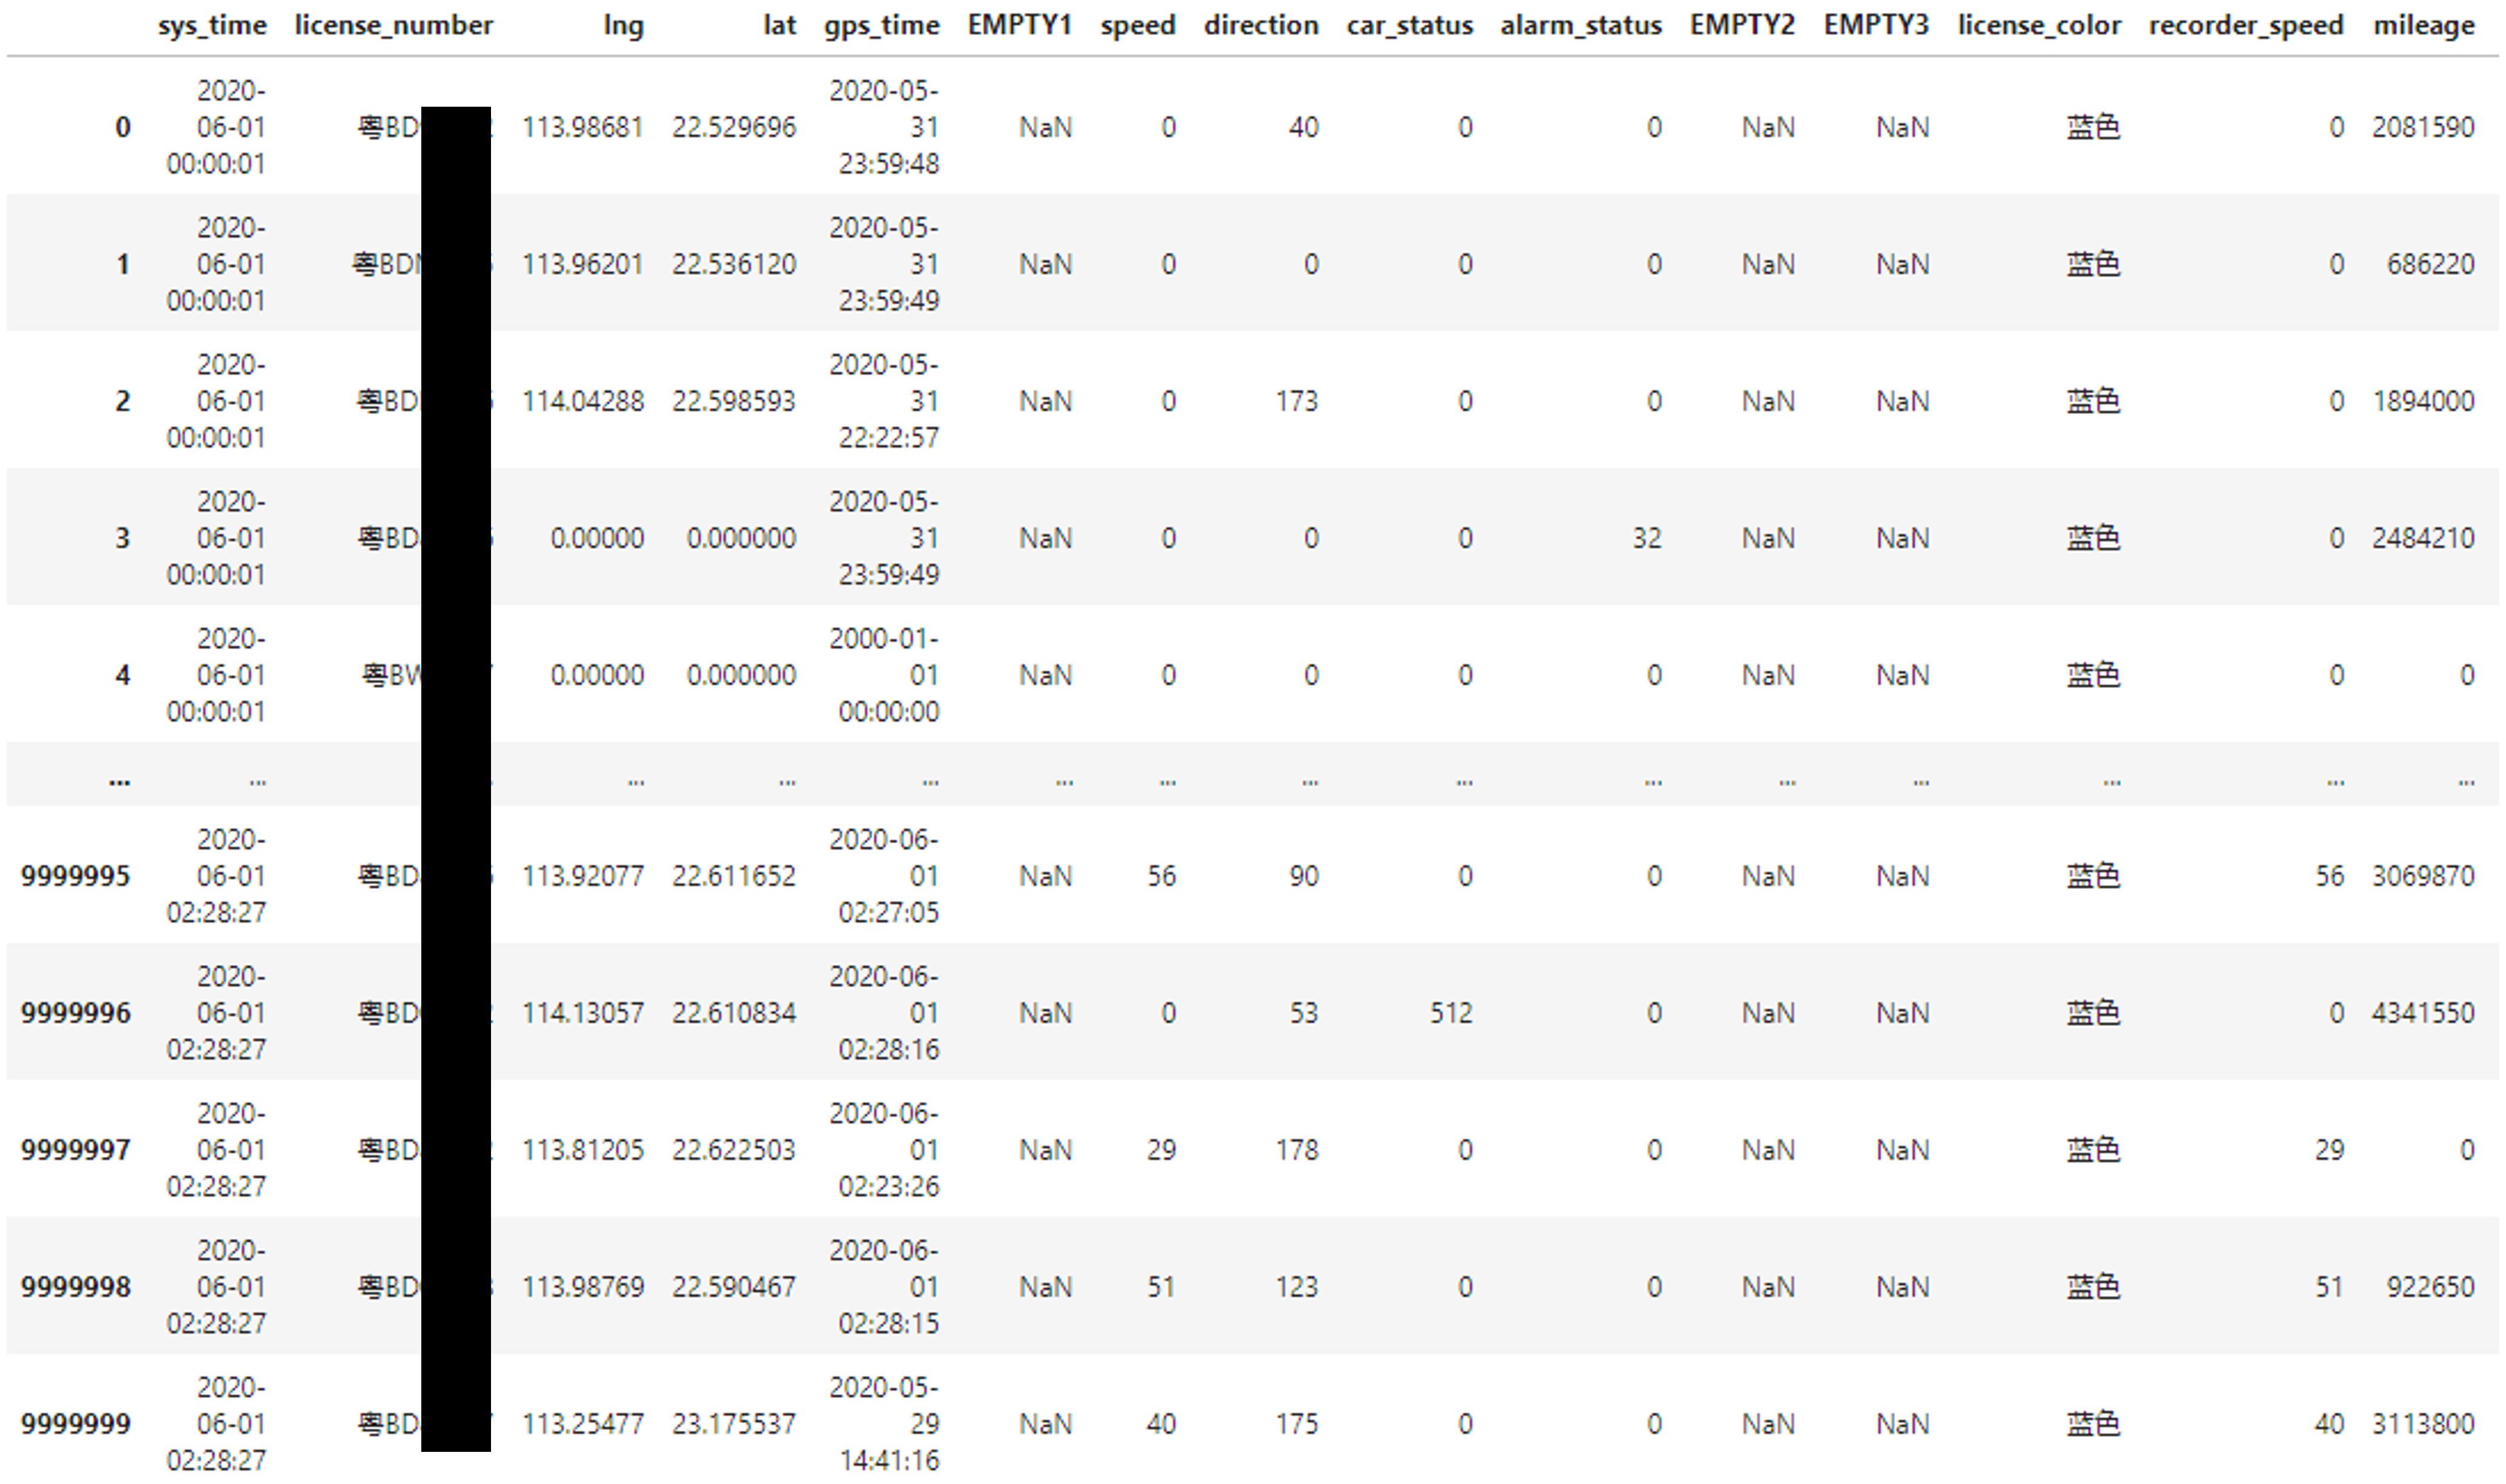
\includegraphics[width=\textwidth]{images/raw_data.png}
    \caption{Shenzhen taxi GPS raw data}
    \label{fig: raw_data}
\end{figure}

Unlike the open datasets that can be applied to deep learning models without the need of data cleaning and completion, this raw dataset contains lots of abnormal values, which should be cleaned and re-organized carefully.

\subsection{Data Cleaning}
Data cleaning is the process of detecting and correcting (or removing) corrupt or inaccurate records from a record set, table, or database and refers to identifying incomplete, incorrect, inaccurate or irrelevant parts of the data and then replacing, modifying, or deleting the dirty or coarse data\cite{data_cleaning}. There are many kinds of bad records that should be deleted or modified. To summarize, we categorize them as the following classes.

\begin{enumerate}
  \item \textbf{Duplicate Rows.} A considerable large part of the raw data are duplicate. The reason is when a GPS device is transmitting data to server, it will send several copies in order to avoid packet loss under poor Internet connection. As a result, they are completely same rows, and thus can be removed safely, leaving only the foremost one.
  \item \textbf{Corrupted Timestamp.} This is a sort of abnormal record. Since our time range is June 2020, all the timestamps that not in here should be deleted. In detail, there are two kinds of them: 1) records in May $31^{st}$ or July $1^{st}$. This is caused by the equipments' lack of accuracy. 2) 2000-01-01. And this is caused by data loss, thus, it is filled by a default value.
  \item \textbf{Abnormal Location.} The latitude and longitude of some records are zero, which is resulted by the data loss during transmission. These dirty values should be deleted.
  \item \textbf{Zero Speed.} Stationary taxis are still transmitting their location information to the server if the GPS device is on, leading to a big portion of zero speed records. They are useless owing to that trajectories are a series of moving locations. Therefore, under normal circumstances, it is better to remove them. However, things are not that happy in our data. There are four kinds of zero speed records relating to the change of location, i.e. latitude and longitude, and they should be treated differently. Details are provided in the next subsection.
  \item \textbf{Irrelevant Attributes.} As shown in figure \ref{fig: raw_data} above, the raw data consists of several columns. The information that have no contribution to trajectories needs to be removed, leaving only latitude, longitude, speed and timestamp.
\end{enumerate}

We take the data of June $1^{st}$ as a case study to give an illustration of our data cleaning procedure. In total, there are 97,453,725 rows.

\begin{table}[htb]
  \begin{center}
      \caption{Data Cleaning Procedure on June $1^{st}$}
      \label{data_cleaning_table}
      \begin{tabular}{ccc}
          \toprule

          \textbf{Action} & \textbf{Deleted Percentage} & \textbf{\#Remaining Rows}\\

          \midrule

          Drop duplicate & $51.73\%$ & 47,042,104\\
          Drop abnormal values & $1.19\%$ & 45,874,548\\
          Drop zero speed & $16.84\%$ & 29,458,603\\

          \cmidrule{1-2}

          \textbf{Remaining Percentage} & $30.22\%$ & ~\\

          \bottomrule
      \end{tabular}
  \end{center}
\end{table}

\subsection{Data Processing}


\section{Methodology}

\subsection{Road Correlation Modeling}

\subsection{Traffic State Prediction}


\section{Experiments}
This is experiments.

\section{Conclusion and Future Work}
This is conclusion.\clearpage

\参考文献
  \printbibliography[heading=none]\clearpage
% \附录
%   \input{sections/examples/appendix.tex}\clearpage
\致谢
  感谢广东省深圳市南山区学苑大道1088号南方科技大学工学院南楼552B崔氏集团实验室
\end{document}